\setchapterstyle{kao}
\setchapterpreamble[u]{\margintoc}
\chapter{Embedding sentences with large transformer models}
%Training sentence embedding models using discriminative objective}
\labch{1B}

\cleanchapterquote{Language is the most interesting manifestation of intelligence. Visual comprehension is something that many animals also have. In some cases, it is even better than that of humans. Chimpanzees also understand feelings and social contexts. But no other living being has such a complex language as we do. And language links all other manifestations of intelligence, because I can talk about what I see, feel and think and how I act.}{Richard Socher}{Interview for \textit{die Zeit}, 2019}
% Artificial Intelligence Doesn't Make After Work Plans
% https://www.zeit.de/digital/2019-05/computational-linguistics-artificial-intelligence-speech-processing-richard-socher?utm_referrer=https%3A%2F%2Ft.co%2F

% \bcomment{you might ask a more incisive question in the first place,suggesstion:}{\ldots }

Bigger is better ? at first sight it seems that current Natural Language Processing is consistently evolving towards larger and larger models paying less and less attention to the models at hand. In this section, we explore how we can leverage the performance of large sentence encoders by adapting their pre-training and increasing their size.

The previous sections discussed the importance of neural model structure in composing sentence representations. Yet, NLP trends do not primarily focus on these types of models, instead focusing on transformers, which are easier to scale. As a result, previous years have seen a general increase in the size of the models and a corresponding improvement over downstream performances. These improvements did not directly benefit sentence embeddings, as many transformer encoders perform below state-of-the-art on standard benchmarks. 
% In this section. we review the challenges and benefits of large models.

This section relates the development of state-of-the-art sentence embedding models as part of the project \textit{Train the Best Sentence Embedding Model Ever with 1B Training Pairs}.\footnote{\url{https://discuss.huggingface.co/t/train-the-best-sentence-embedding-model-ever-with-1b-training-pairs/7354}} This project took place during the \textit{Community week using JAX/Flax for NLP \& CV} organized by Hugging Face.\footnote{\url{https://discuss.huggingface.co/t/open-to-the-community-community-week-using-jax-flax-for-nlp-cv/7104}} Our project was among the competition winners and received an honorable mention. As part of this project, I contributed actively to the construction of the dataset as well as the training and documentation of the sentence embedding models.

We organize the section as follows: we first review the related work and the benefit of scaling in the specific case of sentence embeddings (\refsec{scale:introduction}). \refsec{scale:method} then proposes a self-supervised pre-training approach to learn sentence encoders. The approach addresses engineering challenges such as data collection, framework choice, or training hyper-parameters. Finally, we evaluate the benefit of our approach in \refsec{scale:experiments}.

\section{Transformers and scale}
\labsec{scale:introduction}

Pre-trained transformers resulted in a strong improvement over standard NLP benchmarks. The model \textsc{Bert} indeed claimed a 7.6\% absolute improvement on the popular GLUE benchmark, 5.6\% absolute accuracy improvement on the MultiNLI, and 1.5 F1 points on the SQuAD v1.1 question answering test. \textsc{Bert} introduced many increments to solve NLP tasks, including a new neural architecture, training paradigm number of parameters, and hyper-parameters setup. It is difficult to disentangle the contributions of all these factors, but the number of parameters is one of them. For example, the base version of \textsc{Bert} with 100M parameters achieves an average score of 79.6 on GLUE, while the large version with 340M parameters achieves 82.1. Apart from the number of parameters, the architecture, training procedure, and training data remain unchanged.

Compared with tree-structured encoders, transformers encode sentences without making substantial structure premises. Compared with sequential encoders, they compute each token state simultaneously using the attention mechanism, which is easy to parallelize across computing units. From a computing perspective, transformers are easier to scale. Consequently, the last few years have seen a race to increase the number of layers, parameters, hidden size, or pre-training data size. The model \textsc{Bert} exists in a base and large versions, which only differ by their hidden size and number of parameters. The same is true for the model GPT, which was incremented into GPT-2 and 3. While the second and third versions have much more parameters, the architecture is similar between all versions. As illustrated in \reffig{large-models}, the number of parameters for large language models follows what we may compare with Moore's Law.

% As opposed to deriving complex architectures from linguistic insights. it might be easier to focus on efficient and parallelizable networks. which are easy to scale. 

% Language models also seem to support the adage. "\bcomment{the bigger. the better}{bigger is better}".  The training at scale seems also to leverage some particular behaviors. mediated by some threshold effects. For example \textcite{brown_20} compare generative pre-trained models with distinct sizes on few-shot learning settings. While the smallest model with 1.3B parameters do not show any abilities on the task. the largest model with 175B parameters show surprisingly good generalization performances with a very limited number of training examples.

\begin{figure}[htb!]
	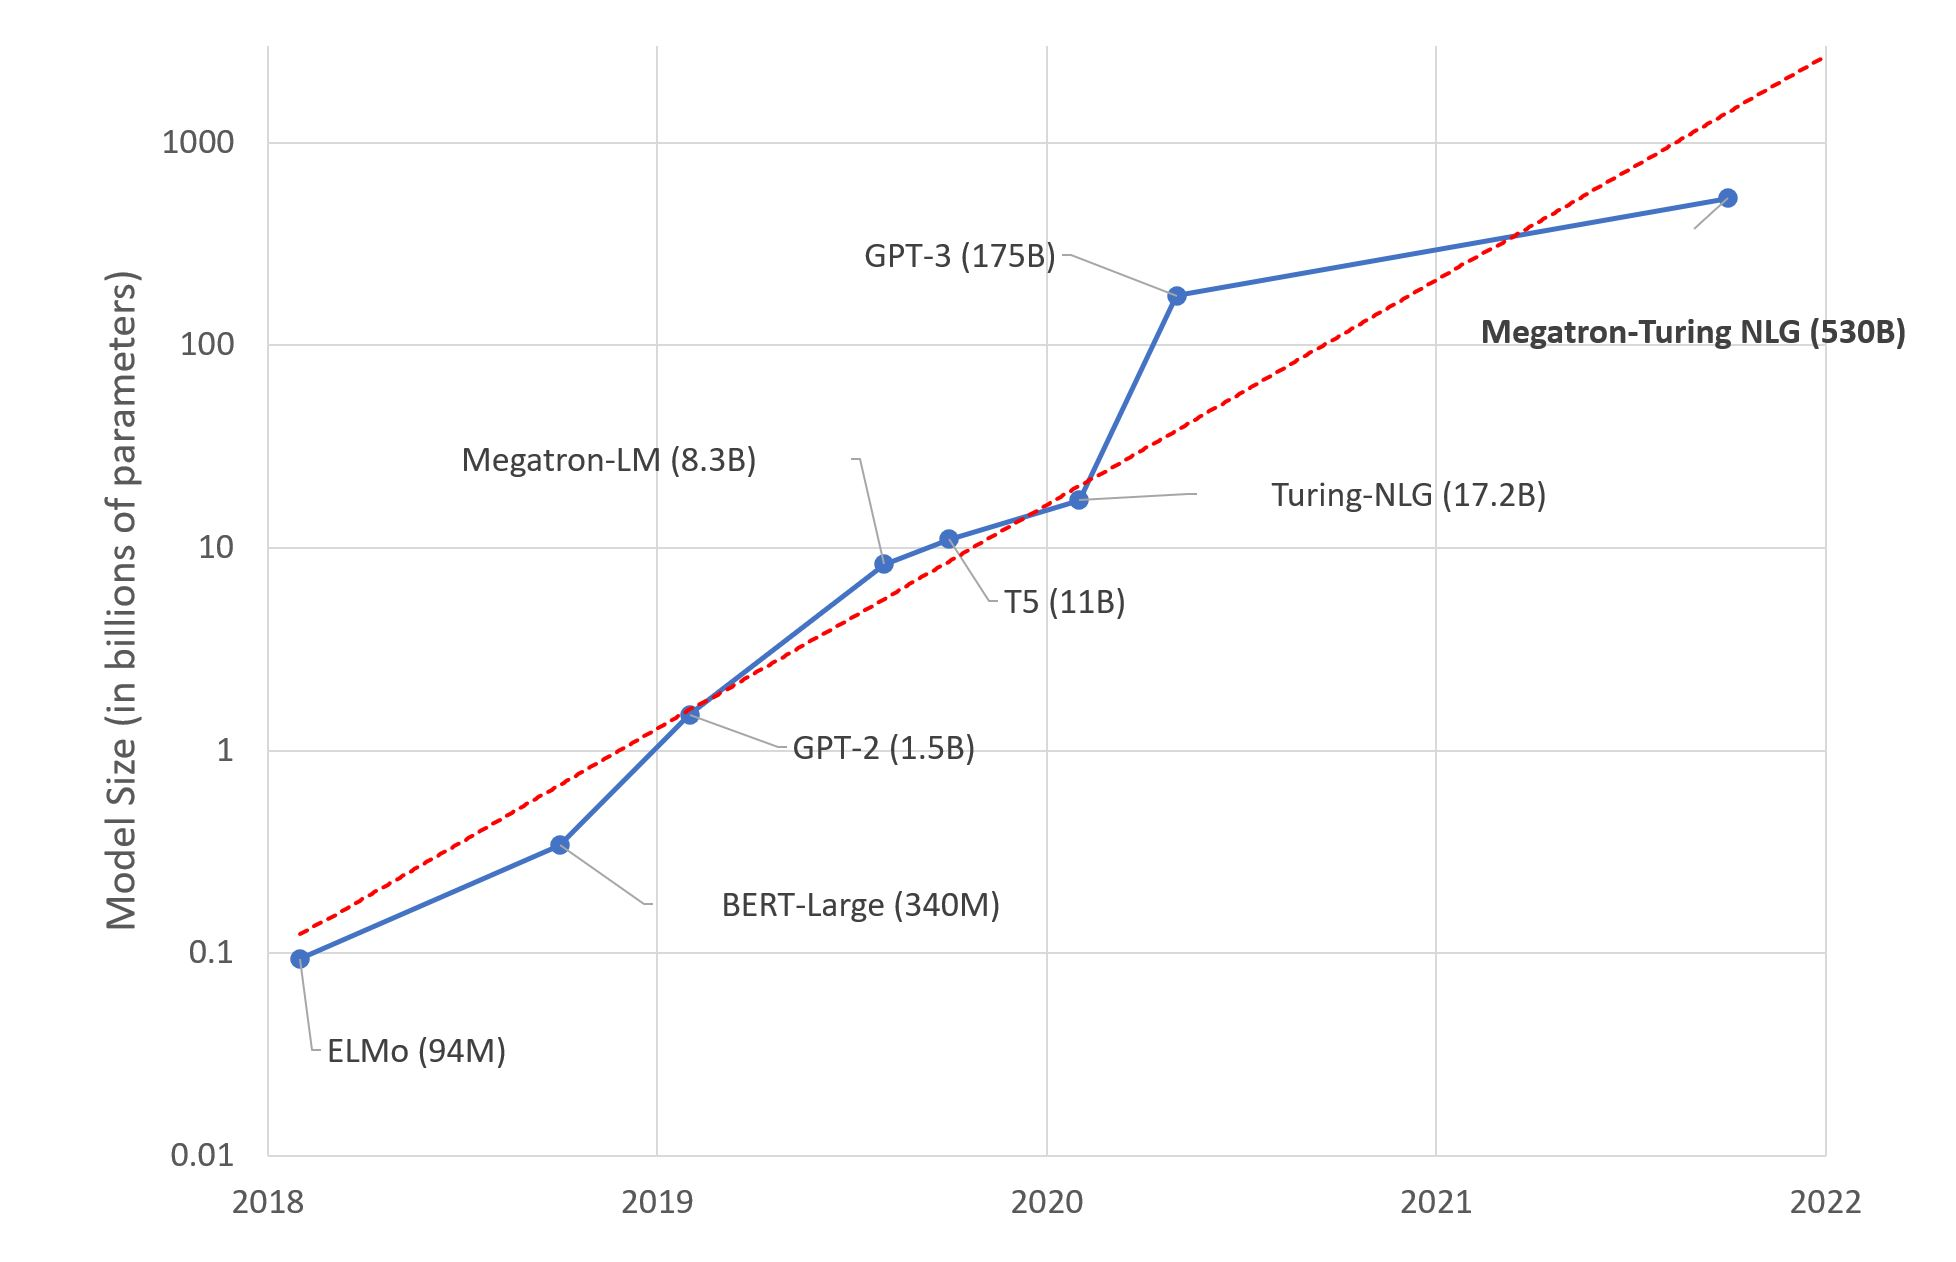
\includegraphics[width=\textwidth]{images/model-size-graph.jpeg}
	\caption[Large models number of parameters]{Evolution of the number of parameters for large language models. The figure is extracted from Microsoft \href{https://www.microsoft.com/en-us/research/blog/using-deepspeed-and-megatron-to-train-megatron-turing-nlg-530b-the-worlds-largest-and-most-powerful-generative-language-model/}{blog post}.}
	\labfig{large-models}
\end{figure}

This analysis also applies in some respects to sentence embeddings. As empirically observed by \textcite{conneau_17}, the embedding size is a key factor in downstream performances over the SentEval benchmark. We reproduce the figure from \textcite{conneau_17} in \reffig{scale:embedding-size}. For almost all encoders shown in the figure, performance increases proportionally to the size of the embeddings. However, regarding specifically \textsc{Bert}, the comparison does not directly extend to the embedding of sentences. Indeed, as already reported in \reftab{contrastive-soa}. \textsc{Bert} performance on the SentEval benchmark is, on average, 3 points below current state-of-the-art methods, including \textcite{simoulin_2021a}.

This lack of performance does not seem to be specifically related to the architecture of transformers. Indeed, \textcite{reimers_19} propose state-of-the-art sentence embeddings by successfully adapting the protocol from \textcite{conneau_17} to transformers. The approach successfully proposes to further fine-tune a pre-trained transformer on natural language inference data.

\begin{figure}[htb!]
	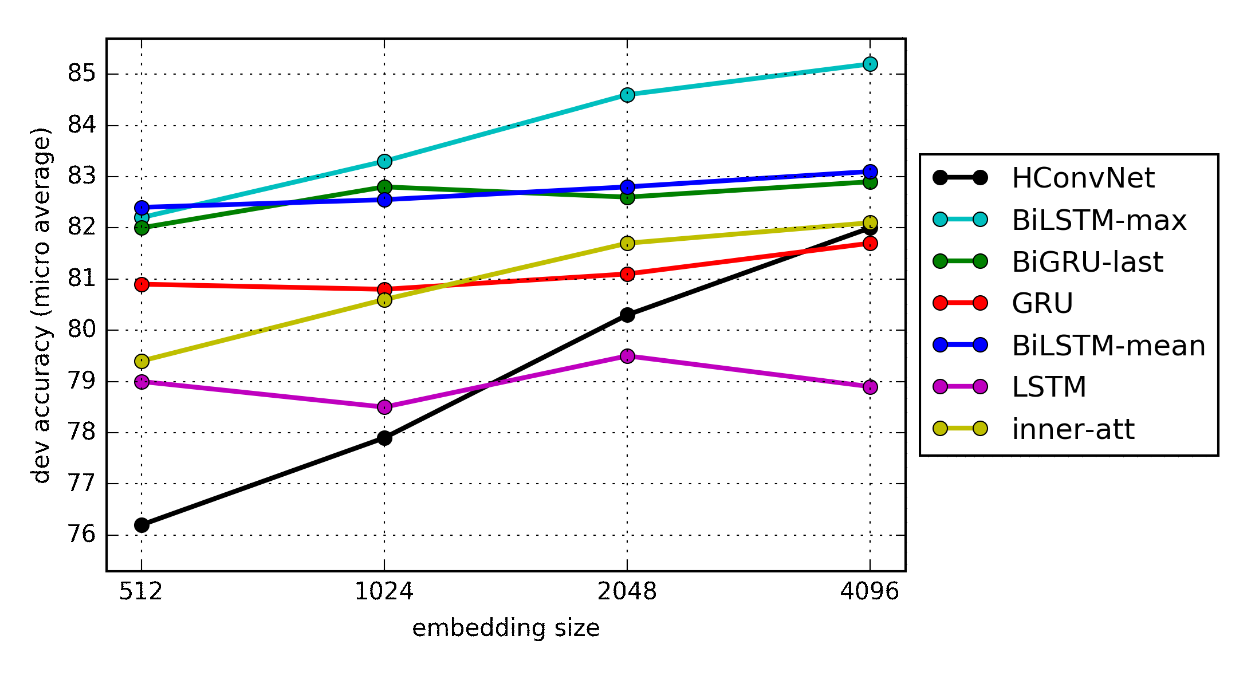
\includegraphics[width=\textwidth]{images/snli_em_size.png}
	\caption{Average performance with respect to the embedding size on the SentEval benchmark. The figure is extracted from \textcite{conneau_17}.}
	\labfig{scale:embedding-size}
\end{figure}

% Here. we study to which extend we can increase sentence encoder performances by scaling their size. As already observed in \refch{arithmetics} or \refsec{survey:downstream}. scaling models is an established method for improving downstream results. However. 

% \bcomment{The previous sections discussed the importance of neural model structure in composing sentence representations. Along with the architecture of the sentence encoder. other parameters may strongly influence the quality of the embeddings. In particular. the last few years have seen a race to increase the number of parameters. hidden size. or size of pre-training data. As already observed in \refch{arithmetics} or \refsec{survey:downstream}. scaling models is an established method for improving downstream results\sidenote{The effect of scaling is considered so obvious that it was used as the primary reason to reject RoBERTa  paper \parencite{liu_2019} from ICLR 2020. As expressed by the Program Chairs: "most of the findings are obvious (careful tuning helps. more data helps)". \url{https://openreview.net/forum?id=SyxS0T4tvS}}.}{manque de problématique; ne pas mettre cette note en évidence}


% \section{Train a sentence embedding model with 1 billion training pairs}
% \labsec{1B}

\section{Method}
\labsec{scale:method}

Even though the effect of scaling is no longer a surprise, training large models continues to be a challenging exercise. Training large models poses engineering challenges for optimization \parencite{you_20}, infrastructure \parencite{shoeybi_19, narayanan_21} or data collection \parencite{OrtizSuarezSagotRomary2019}.

\subsection{Training objective}
\labsec{1B:objective}

As in \refch{structure-scale}, we use a contrastive objective to train our sentence encoders. We collect sentence pairs $(a_i, p_i)$ that are somehow semantically related. The effective construction of the dataset is detailed in \refsec{1B:dataset}. We train the model to map pairs $(a_i, p_i)$ to close vectors while assigning unmatched pairs $(a_i, p_j)_{i \neq j}$ to distant vectors in the embedding space. This training method closely relates Quickthought (presented in \refsec{training}), contrastive unsupervised representation learning \parencite{saunshi_19}, training with in-batch negatives \parencite{carlsson_21}, InfoNCE \parencite{oord_18} or NTXentLoss \parencite{sohn_16}.

We illustrate the training objective in \reffig{contrastive}. Intuitively, the model should assign high similarity to the sentences « How many people live in Berlin? » and « Around 3.5 million people live in Berlin » and low similarity to other negative answers such as « The capital of France is Paris ».

\begin{figure}[htb!]
	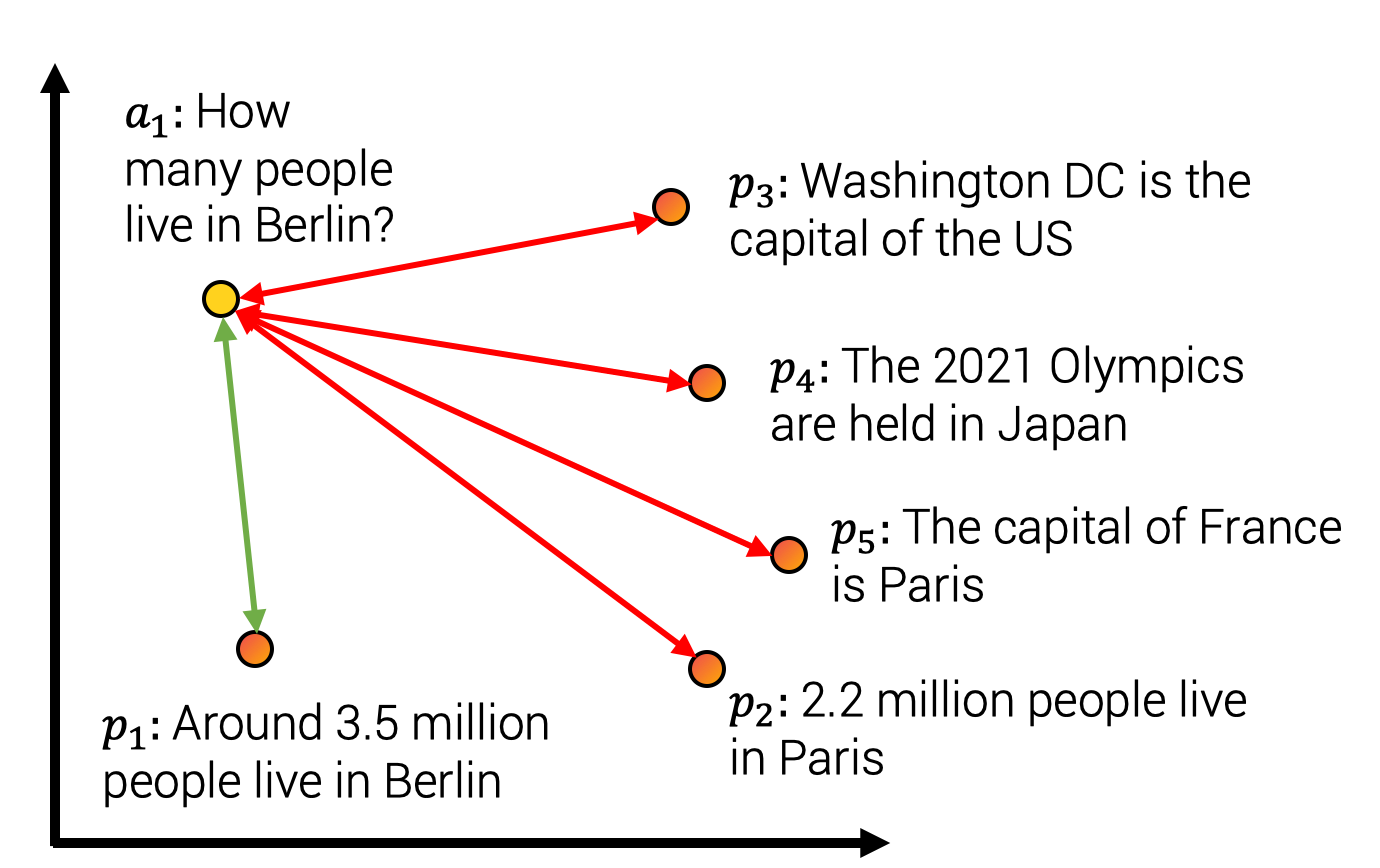
\includegraphics[width=10cm]{images/contrastive_1.png}
	\caption[Contrastive learning]{Illustration of the contrastive learning setup. The model is trained to associate an anchor sentence with another one that is semantically related. The notion of semantic relation depends on the nature of the pair. Our example aims to link the correct answer to a given question. City capitals are the subject of all these sentences, but only one is the correct answer.}
	\labfig{contrastive}
\end{figure}

As in other contrastive methods detailed in \refsec{training:self-supervised}, we build negative pairs by considering other samples from the batch. Given a batch of $n$ training samples, the model optimizes the following loss function:

\begin{equation}
    \mathcal{L} = -\frac{1}{n}\sum_{i=1}^n\frac{e^{c(a_i. p_i)}}{\sum_j e^{c(a_i. p_j)}}    
\end{equation}

Where $c$ is a \textit{critic function}, which measures the distance between two sentence embeddings $(a, p)$.\sidenote{A set of possible critics is presented in \cite{tschannen_19} Most functions are either the cosine similarity or the dot product operator. The cosine similarity has the nice advantage of presenting the highest similarity to itself since $cos(a, a) =1$. While with the dot-product other vectors can have higher similarities: $dot(a, a) < dot (a, b)$.}.

%We illustrate the training objective in \reffig{contrastive-2}.

% \begin{figure}[htb!]
% 	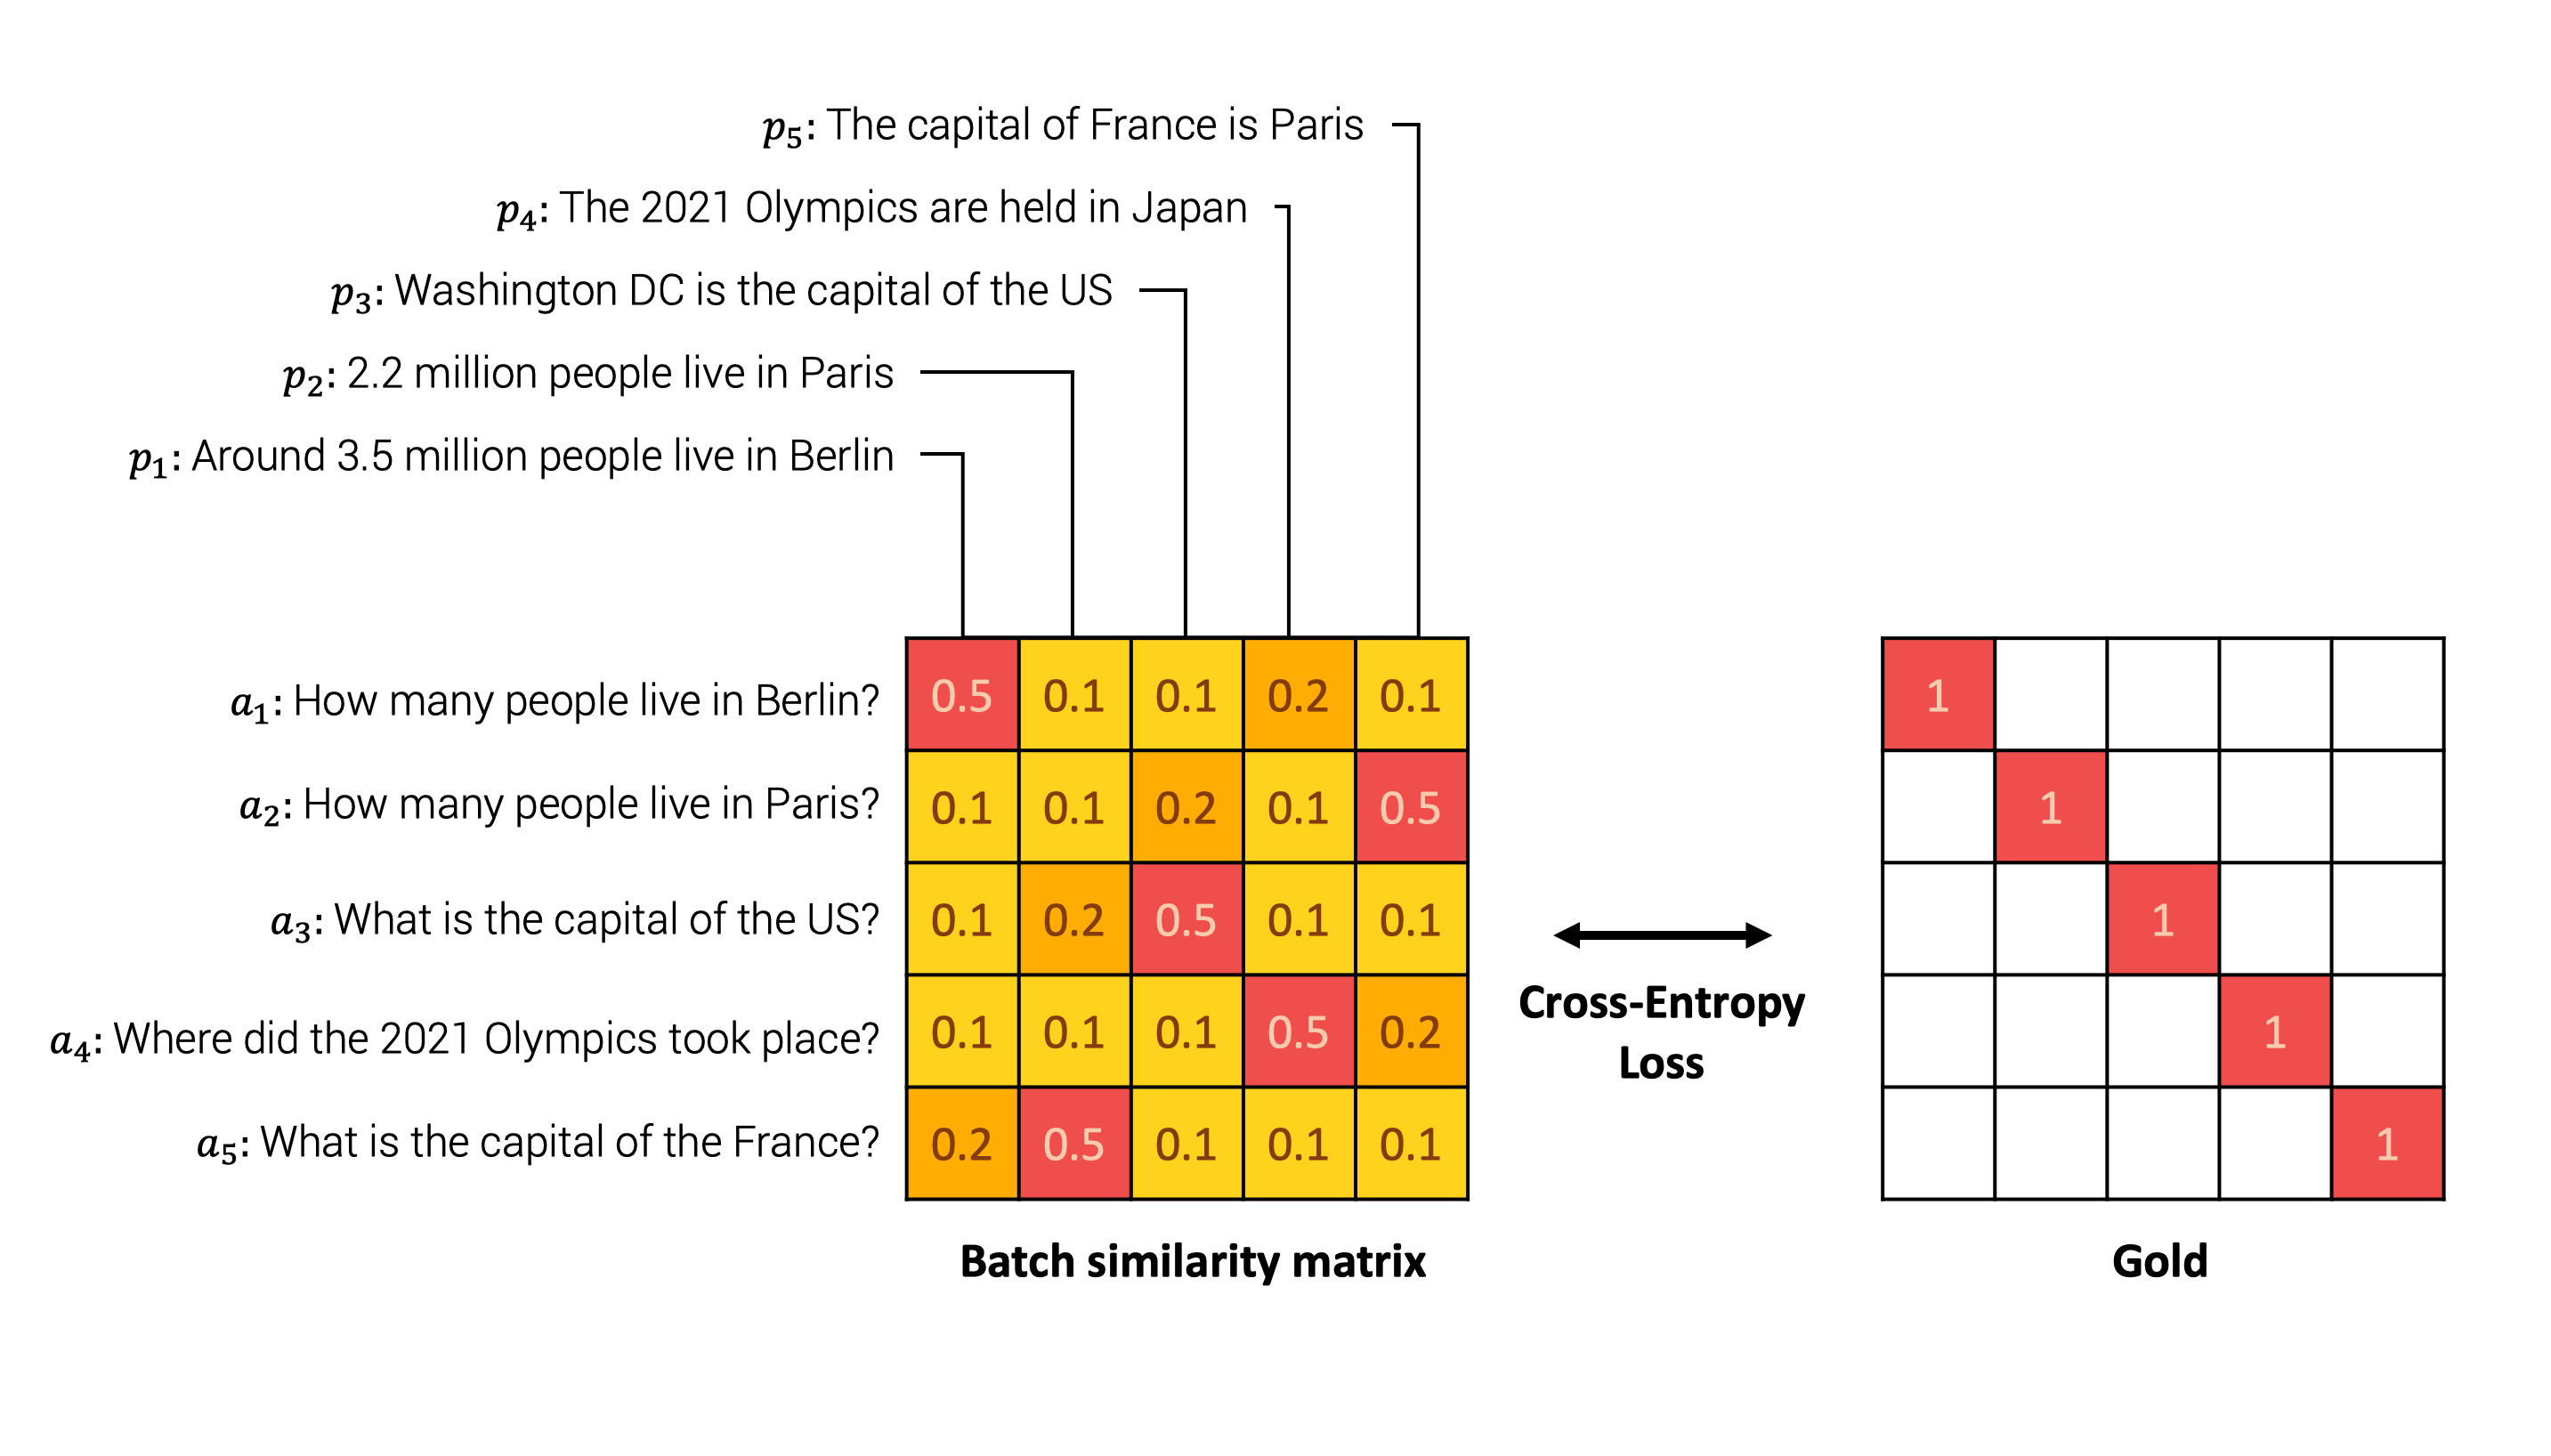
\includegraphics[width=10cm]{images/contrastive_2.png}
% 	\caption[Contrastive learning]{Illustration of the contrastive learning objective.}
% 	\labfig{contrastive-2}
% \end{figure}

\subsection{Construction of the dataset}
\labsec{1B:dataset}

The contrastive training method supposes to build a dataset such that each sample $x$ is combined with another sample $x^+$, which is somehow \textit{close} and negative samples $s^-_1 \cdots s^-_K$, which are not related. In \refch{structure-scale}, we constructed positive pairs by simply associating context sentences and negative by considering non-context sentences. Therefore, we only needed a corpus of raw text for which the sentence order is preserved to train our model. In this experiment, we adopt a more refined approach. Instead of raw text, we extract sentences from specific mediums such as internet forums or manually labeled datasets. Indeed, as detailed in \refsec{1B:batches}, a better selection of negative samples may drastically increase the results.

As with other attempts to scale model size \parencite{liu_2019, radford_2019, brown_20}, we also aim to scale the dataset size. While we use a 40M sentences dataset for \textcite{simoulin_2021a}, here, we aim to gather a dataset of 1B sentence pairs. The task is far from trivial as we need to constitute a dataset with sentence pairs $(a_i, p_i)$ such that sentences from the pair have a close meaning. We constitute pairs by using  medium and documents specific structure such as (query, answer-passage), (question, duplicate\_question), (paper title, cited paper title). We do not build new datasets but instead rely on existing work and aggregat many existing datasets enumerated in \reftab{tab:1B:dataset}.

The majority of the datasets is built out of Reddit comments. Reddit website aggregates news and lets users post links and discuss through threads. We use scripts from PolyAI to generate tuples given the first comment for each response.\sidenote{\url{https://github.com/PolyAI-LDN/conversational-datasets/tree/master/reddit}} We use the same filters as \textcite{henderson_2019} and filter out samples with more than 128 characters or fewer than 9 characters. I personally took care of this data collection operation.

\begin{table*}[!htb]
\centering
\footnotesize
\begin{tabularx}{16cm}{@{}lp{4.5cm}Y@{} }
\toprule
\textbf{Dataset} & \textbf{Reference} & \textbf{Number of training pairs} \\
\midrule
\midrule 
\href{https://github.com/PolyAI-LDN/conversational-datasets/tree/master/reddit}{Reddit Comments} (2015-2018) & \textcite{henderson_19} & \num{726484430} \\
\href{https://github.com/allenai/s2orc}{S2ORC} citation pairs (abstracts) & \textcite{lo_20} & \num{116288806} \\
\href{https://github.com/afader/oqa\#wikianswers-corpus}{WikiAnswers} duplicate question pairs & \textcite{fader_14} & \num{77427422} \\
\href{https://github.com/facebookresearch/PAQ}{PAQ} (question. answer) pairs & \textcite{lewis_21} & \num{64371441} \\
\href{https://github.com/allenai/s2orc}{S2ORC} citation pairs (titles) & \textcite{lo_20} & \num{52603982} \\
\href{https://github.com/allenai/s2orc}{S2ORC} (title. abstract) & \textcite{lo_20} & \num{41769185} \\
\href{https://huggingface.co/datasets/flax-sentence-embeddings/stackexchange_xml}{Stack Exchange} (title. body) pairs & - & \num{25316456} \\
\href{https://microsoft.github.io/msmarco/}{MS MARCO} triplets & \textcite{craswell_21} & \num{9144553} \\
\href{https://github.com/allenai/gooaq}{GOOAQ} & \textcite{khashabi_21} & \num{3012496} \\
\href{https://www.kaggle.com/soumikrakshit/yahoo-answers-dataset}{Yahoo Answers} (title. answer) & \textcite{zhang_15} & \num{1198260} \\
\href{https://huggingface.co/datasets/code_search_net}{Code Search} & - & \num{1151414} \\
\href{https://cocodataset.org/\#home}{COCO} image captions & \textcite{lin_14} & \num{828395} \\
\href{https://github.com/allenai/specter}{SPECTER} citation triplets & \textcite{cohan_20} & \num{684100} \\
\href{https://www.kaggle.com/soumikrakshit/yahoo-answers-dataset}{Yahoo Answers} (question. answer) & \textcite{zhang_15} & \num{681164} \\
\href{https://www.kaggle.com/soumikrakshit/yahoo-answers-dataset}{Yahoo Answers} (title. question) & \textcite{zhang_15} & \num{659896} \\
\href{https://huggingface.co/datasets/search_qa}{SearchQA} & \textcite{dunn_17} & \num{582261} \\
\href{https://huggingface.co/datasets/eli5}{Eli5} & \textcite{fan_19} & \num{325475} \\
\href{https://shannon.cs.illinois.edu/DenotationGraph/}{Flickr 30k} & \textcite{young_14} & \num{317695} \\
\href{https://huggingface.co/datasets/flax-sentence-embeddings/stackexchange_xml}{Stack Exchange} duplicate questions (titles) & - & \num{304525} \\
AllNLI (\href{https://nlp.stanford.edu/projects/snli/}{SNLI} and \href{https://cims.nyu.edu/~sbowman/multinli/}{MultiNLI}) & \textcite{bowman_15, williams_18b} & \num{277230} \\
\href{https://huggingface.co/datasets/flax-sentence-embeddings/stackexchange_xml}{Stack Exchange} duplicate questions (bodies) & - & \num{250519} \\
\href{https://huggingface.co/datasets/flax-sentence-embeddings/stackexchange_xml}{Stack Exchange} duplicate questions (titles and bodies) & - & \num{250460} \\
\href{https://github.com/google-research-datasets/sentence-compression}{Sentence Compression} & \textcite{filippova_13} & \num{180000} \\
\href{https://github.com/pvl/wikihow_pairs_dataset}{Wikihow} & \textcite{koupaee_18} & \num{128542} \\
\href{https://github.com/chridey/altlex/}{Altlex} & \textcite{hidey_16} & \num{112696} \\
\href{https://quoradata.quora.com/First-Quora-Dataset-Release-Question-Pairs}{Quora Question Triplets} & - & \num{103663} \\
\href{https://cs.pomona.edu/~dkauchak/simplification/}{Simple Wikipedia} & \textcite{coster_11} & \num{102225} \\
\href{https://ai.google.com/research/NaturalQuestions}{Natural Questions (NQ)} & \textcite{kwiatkowski_19} & \num{100231} \\
\href{https://rajpurkar.github.io/SQuAD-explorer/}{SQuAD2.0} & \textcite{drajpurkar_18} & \num{87599} \\
\href{https://huggingface.co/datasets/trivia_qa}{TriviaQA} & - & \num{73346} \\
\midrule
\textbf{Total} & & \textbf{\num{1124818467}} \\
\bottomrule
\end{tabularx}
\caption{1 billion sentence pairs dataset. We use already existing datasets accessible in open source or for which the raw data and pre-processing scripts were available. For each sub-dataset, we provide the link to the available resources (existing dataset or pre-processing scripts).}
\labtab{tab:1B:dataset}
\end{table*}

\subsection{Construction of the mini batches}
\labsec{1B:batches}

When building models. the selection of pairs forming a batch is crucial. We present here our strategy to constitute mini-batches and the impact it may have on the resulting embeddings.
% Here we examine the batch characteristics and their impact on the embeddings.

\paragraph{Batch size} The Quickthought method detailed in \refsec{training:self-supervised} uses a rather important batch size of 400. In fact, studies show that the more large the batch, the better the performances  \parencite{chen_20a, qu_21}. This trend is illustrated \reffig{batch-size} extracted from \textcite{qu_21}. Yet, too important batch size may decrease the results (the same asymptotic phenomenon is observed in \textcite{chen_20a}). We benefited from efficient hardware infrastructure to run the project: 7 TPUs v3-8, as well as guidance from Google’s Flax, JAX, and Cloud team members about efficient deep learning frameworks. We use the largest batch size that our hardware could fit, in our case, 64.

\begin{figure}[htb!]
	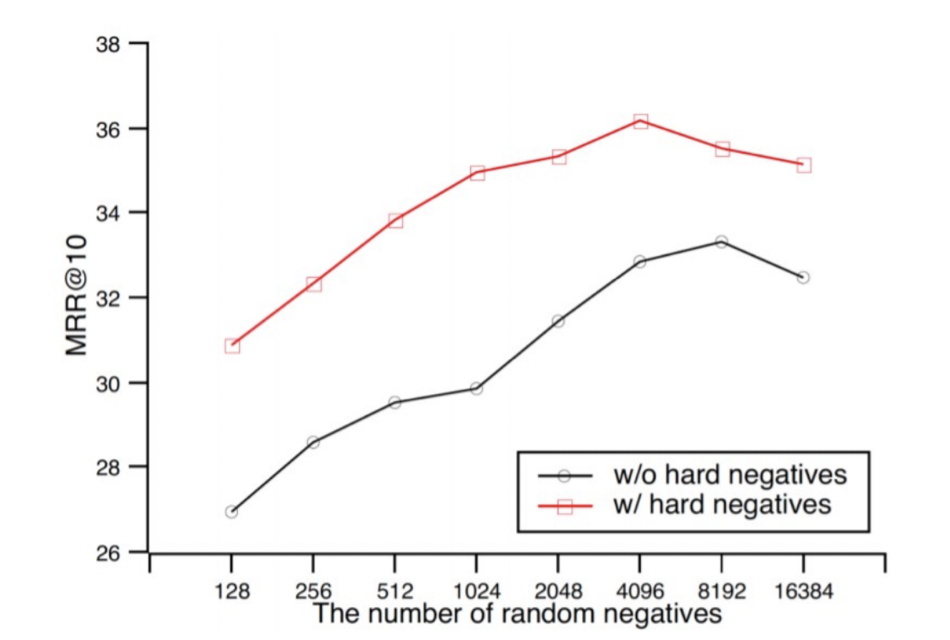
\includegraphics[width=10cm]{images/batch-size.png}
	\caption[Batch size]{Influence from the batch size and selection of hard negative on downstream evaluation. The figure is extracted from \textcite{qu_21}.}
	\labfig{batch-size}
\end{figure}

\paragraph{Hard Negatives} We may build batches by uniformly selecting samples from the training data. Yet, as detailed in \textcite{robinson_21} or \textcite{qu_21}. the selection of "good negative examples" significantly impacts the training process. The impact of hard negative is illustrated in \reffig{batch-size}.
Hard negative examples should not correspond to the anchor point but still, be difficult to distinguish from the correct associations. 
% Hard negatives are sample $p_j$. which are hard to distinguish from $p_i$. 
In our example, it could be the pairs « What is the capital of France? » and « What is the capital of the US? » which have a close semantic content and requires precisely understanding the full sentence to be answered correctly. On the contrary, the samples « What is the capital of France? » and «How many Star Wars movies are there?» are less difficult to distinguish since they do not refer to the same topic.

\paragraph{Cross dataset batches} In our case, the dataset is a concatenation of several sub-datasets (\reftab{tab:1B:dataset}). Each sub-dataset is built on distinct topics, domains, or semantic relations in the pair. We want to avoid the case where our model learns disjoint embedding spaces for each sub-dataset. On the other hand, mixing all sub-datasets in the same batch may deteriorate the hard negative proportion as samples issued from two sub-datasets should be easy to differentiate. To address both requirements, we build batches from the mix of only two sub-datasets. We aim, therefore, to learn a global structure between topics and not only a local structure within a topic while not deteriorating the proportion of hard negatives.

\subsection{Evaluation}
\labsec{scale:evaluation}

As detailed in \refsec{survey:downstream}, sentence embeddings are traditionally evaluated on the SentEval benchmark. To compare the embeddings with models developed in previous sections, we, therefore, evaluate our encoders on SentEval. However, as detailed in the same section, the benchmark suffers from practical limitations or biases. For this project, we, therefore, used SEB (Sentence Embedding Benchmark), a dedicated benchmark to compare our models.\sidenote{\url{https://github.com/nreimers/se-benchmark}} The SEB benchmark aggregates multiple general-purpose sentence evaluation tasks. The tasks, detailed below, are formatted as binary classification, clustering, reranking, retrieval, and semantic textual similarity (STS). All tasks use the embeddings as features and compare them using similarity metrics. Most importantly, they do not require the training of additional classifiers.

\paragraph{Binary classification} aims at predicting a binary relation between a pair of sentences. It computes the cosine similarity between every pair of sentences. We then classify the sentence pairs by comparing their similarity score to a given threshold. We set the threshold to ensure the best score on the development set. The task includes identifying paraphrases from LanguageNet, a collection of sentences from Twitter linked through shared URLs \sidenote{\url{https://languagenet.github.io/}} or the SemEval-2015 Task 1,\sidenote{\url{https://alt.qcri.org/semeval2015/task1/}} and identifying duplicated questions.\sidenote{\url{https://www.aclweb.org/anthology/D18-1131/}} We measure the performances using the average precision (AP).\sidenote{The average precision (AP) has values between 0 and 1 (higher is better). AP is defined as $\sum_n(R_n-R_{n-1})P_n$ with $P_n$ and $R_n$ are the precision and recall at the nth threshold. \url{https://scikit-learn.org/stable/modules/generated/sklearn.metrics.average_precision_score.html}}

\paragraph{Clustering} organizes documents into semantically consistent groups. We use data from web forums and newsgroups, which organizes posts given their topics. We use embeddings as features for K-Means clustering and evaluation using the V-measure.\sidenote{The V-measure evaluates the quality of a clustering given the ground truth labels. The score has positive values between 0 and 1, with higher values indicating better results. The V-measure is the harmonic mean between homogeneity and completeness. Homogeneity evaluates if each cluster contains only members of a single class. Completeness determines if all members of a class are assigned to the same cluster. \url{https://scikit-learn.org/stable/modules/generated/sklearn.metrics.v_measure_score.html}} The clustering task includes the 20Newsgroups,\sidenote{\url{https://scikit-learn.org/0.19/datasets/twenty_newsgroups.html}} and clustering threads from StackExchange and Reddit. 

\paragraph{Retrieval} aims at retrieving documents from a corpus that match the semantic content of a given query. We use datasets scraped from web forums and question-answering websites. On such platforms, experienced users can flag a question as a duplicate if it has already been answered elsewhere. We use these annotations to associate a given question to a list (of variable size) of semantically equivalent formulations. Given the embedding of a query, we compute the cosine similarity with other questions from the dataset and retrieve the top-$k$ most similar ones (by default, we use $k=10$). We then compare our predicted list with the related questions using the Mean average precision (MAP@100). The task includes CQADupStack, a dataset with duplicate question information from StackExchange subforums\sidenote{\url{http://nlp.cis.unimelb.edu.au/resources/cqadupstack/}} and the Quora Question Pairs dataset.\sidenote{\url{https://quoradata.quora.com/First-Quora-Dataset-Release-Question-Pairs}}
%  the Mean Reciprocal Rank (MRR) or 

\paragraph{Reranking} ranks a list of documents given their semantic similarity with a given query. In our setup, the task takes a query and a fixed-length list of documents as input. Each document in the list is either "similar" or "non-similar" to the query. We compute the cosine similarity between the embedding of the query and each document and sort them in decreasing order. We then compare the sorted list with the document ordered as similar first, followed by non-similar. We also use mean average precision to measure the quality of the ranking. As in the retrieval task, data are collected from web forums but with a different format and labeling process. We use a collection of questions taken from AskUbuntu.com 2014 corpus dump.\sidenote{\url{https://github.com/taolei87/askubuntu}} SciDocs. which consider scientific papers as related based on their inter citations \sidenote{\url{https://allenai.org/data/scidocs}} and the Stack Overflow Duplicate Questions Task.\sidenote{\url{https://www.microsoft.com/en-us/research/uploads/prod/2019/03/nl4se18LinkSO.pdf}}

\paragraph{Semantic Textual Similarity (STS)} measures the semantic similarity between two sentences. Annotators assign a similarity score for pair of sentences, ranging from 0 for no overlap to 5 for meaning equivalence. The annotation doesn't require formal linguistic expertise. Performance compares the correlation between predicted scores and human judgments with Pearson correlation. The predicted scores directly measure the cosine similarity between two sentence pairs and compare it with human gold annotations (scaled between 0 and 1). The evaluation datasets include the STSBenchmark\sidenote{\url{http://ixa2.si.ehu.eus/stswiki/index.php/STSbenchmark}} which includes datasets used for the SemEval task from 2012 to 2017. the SICK-R task (already introduced in \refsec{sts}) and BIOSSES \sidenote{\url{https://tabilab.cmpe.boun.edu.tr/BIOSSES/DataSet.html}} which comprises 100 sentence pairs from the biomedical field.

% \begin{table}[ht!]
% \begin{center}
% \small
% {\renewcommand{\arraystretch}{1.25}
% \begin{tabular}{|c|p{0.88\linewidth}|}
% \hline
% \multirow{4}{*}{5}& \emph{The two sentences are completely equivalent. as they mean the same thing.}\\
% \cline{2-2}
% & The bird is bathing in the sink. \newline Birdie is washing itself in the water basin. \\
% \hline
% \multirow{4}{*}{4}  & \emph{The two sentences are mostly equivalent. but some {\it unimportant} details differ.}\\
% \cline{2-2}
% & Two boys on a couch are playing video games. \newline Two boys are playing a video game. \\
% \hline
% \multirow{4}{*}{3} & \emph{The two sentences are roughly equivalent. but some {\it important information} differs/missing.}\\
% \cline{2-2}
% & John said he is considered a witness but not a suspect. \newline ``He is not a suspect anymore.'' John said.  \\
% \hline
% \multirow{4}{*}{2} & \emph{The two sentences are not equivalent. but share some details.}\\
% \cline{2-2}
% & They flew out of the nest in groups. \newline They flew into the nest together. \\
% \hline
% \multirow{4}{*}{1} & \emph{The two sentences are not equivalent. but are on the same topic.}\\
% \cline{2-2}
% & The woman is playing the violin. \newline The young lady enjoys listening to the guitar. \\
% \hline
% \multirow{4}{*}{0} & \emph{The two sentences are completely dissimilar.}\\
% \cline{2-2}
% & The black dog is running through the snow. \newline A race car driver is driving his car through the mud. \\
% \hline
% \end{tabular}
% }
% \end{center}
% \caption{Similarity scores with explanations and English examples. The table is exctracted from \textcite{cer_17}.}
% \label{fig:annotationcore}
% \end{table}

\section{Experiments}
\labsec{scale:experiments}

We fine-tune existing pre-trained models with our contrastive learning objective. As a sentence representation, we take the mean of every token hidden state from transformer models. We applied 500 warm-up steps and use a batch size of 64 if not explicitly specified otherwise. We create 20 general-purpose sentence transformers models such as Mini-LM \parencite{wang_20a}. RoBERTa \parencite{liu_2019}. DistilRoBERTa. a distilled version of the RoBERTa-base model following the same training procedure as DistilBERT \parencite{sanh_19}. and MPNet \parencite{song_20}.\sidenote{All models created during the challenge are available as open-source contributions in our HuggingFace repository \url{https://huggingface.co/flax-sentence-embeddings}.} The challenge was limited in time, and we could not extensively train all models with the same number of steps. We train RoBertA-large and MPNet-base for 400k steps. Mini-LM-12 for 540 steps. RoBERTa-distill-base for 920 steps and Mini-LM-6 for \numprint{1000} steps. Yet, models may therefore not be directly compared.



\paragraph{Analysis of the pre-training} We evaluate all our models on the Sentence Embedding Benchmark (SEB) detailed in \refsec{scale:evaluation} and SentEval benchmark introduced in \refsec{survey:downstream}. \reftab{scale:seb-senteval} reports the mean score for each model on both benchmarks. For each model, we report the score for the raw model and for the model further tuned with our additional contrastive pre-training.

\begin{table*}[!htb]
\centering
\small
\begin{tabularx}{16cm}{@{}lYYYYY@{} }
\toprule
&  & \multicolumn{2}{c}{\textbf{SentEval}} & \multicolumn{2}{c}{\textbf{SEB}}\\
\textbf{Model} & \textbf{\# parameters} & w/o contrastive pre-training & w/ contrastive pre-training & w/o contrastive pre-training & w/ contrastive pre-training\\
\midrule
\midrule 
\href{https://huggingface.co/flax-sentence-embeddings/all_datasets_v4_MiniLM-L6}{Mini-LM-6} & 22.7M & 80.6 & 83.5 & 42.0 & 68.1 \\
\href{https://huggingface.co/flax-sentence-embeddings/all_datasets_v4_MiniLM-L12}{Mini-LM-12} & 33.4M & 81.7 & 84.8 & 40.7 & 68.6 \\
\href{https://huggingface.co/flax-sentence-embeddings/all_datasets_v3_distilroberta-base}{DistilRoBERTa} & 82.1M & 83.5 & 86.0 & 44.9 & 68.7 \\
\href{https://huggingface.co/flax-sentence-embeddings/all_datasets_v4_mpnet-base}{MPNet-base} & 109.5M & \textbf{83.5} & \textbf{87.4} & 41.6 & 69.5 \\
\href{https://huggingface.co/flax-sentence-embeddings/all_datasets_v3_roberta-large}{RoBERTa-large} & 355.4M & 81.7 & 87.3 & \textbf{45.3} & \textbf{70.0} \\
\bottomrule
\end{tabularx}
\caption{\labtab{scale:seb-senteval} Evaluation on SentEval and SEB. We report the mean score over all tasks from the benchmark. We compare models pre-trained with and without our contrastive procedure. We report the best results for each category in \textbf{bold}.}
\end{table*}

In general, transformer models with a higher number of parameters reach higher scores. Yet, we observe asymptotic behavior for this trend. The RoBERTa-large model reaches performances similar to MPNet-base despite having 3 times more parameters. Moreover, on both benchmarks, the contrastive pre-training procedure has an important impact. Model performances increase up to 5.6 points on SentEval and more than 20 points on SEB. This confirms the relevance of the procedure for training sentence encoders with transformer architectures. Finally, we observe less disparity between models on the SEB benchmarks for which all scores are very close. 

\paragraph{Sentence Embedding Benchmark (SEB)} \reftab{scale:seb} reports the detailed evaluation of our models on SEB. The results are more difficult to interpret. While larger models tend in general to perform better, no model seems to consistently outperform others. It is also difficult to identify specifics models behavior across task classes.

\setlength\tabcolsep{2pt} % default value: 6pt
\begin{table*}[!htb]
\footnotesize
\centering {
\begin{tabularx}{16cm}{@{}l Y Y Y | Y Y Y | Y Y | Y Y Y | Y Y Y@{}}
\toprule
& \multicolumn{3}{c}{\textbf{Binary Classification}} & \multicolumn{3}{c}{\textbf{Clustering}} & \multicolumn{2}{c}{\textbf{Retrieval}} & \multicolumn{3}{c}{\textbf{Re-ranking}} & \multicolumn{3}{c}{\textbf{STS}}\\
& {\tiny\textbf{Sprint}} & {\tiny\textbf{Twitter}} & {\tiny\textbf{SemEval}} & {\tiny\textbf{20 News Groups}} & {\tiny\textbf{Stack Exchange}} & {\tiny\textbf{Reddit}} & {\tiny\textbf{CQA}} & {\tiny\textbf{Quora}} & {\tiny\textbf{Ask Ubuntu}} & {\tiny\textbf{Sci Docs}} & {\tiny\textbf{Stack Overflow}} & {\tiny\textbf{SICK-R}} & {\tiny\textbf{STS}} & {\tiny\textbf{BIOSSES}}\\\midrule
\midrule
\href{https://huggingface.co/flax-sentence-embeddings/all_datasets_v4_MiniLM-L6}{Mini-LM-6} & \textbf{94.6} & 84.7 & 67.9 & 46.2 & 54.4 & 50.2 & 28.6 & 84.9 & 63.5 & 87.1 & 50.8 & 77.2 & 82.0 & 81.6 \\
\href{https://huggingface.co/flax-sentence-embeddings/all_datasets_v4_MiniLM-L12}{Mini-LM-12} & 92.6 & 84.8 & 70.0 & 46.9 & 52.4 & 50.6 & 29.4 & \textbf{85.1} & 64.1 & 87.2 & 51.5 & 78.9 & 83.1 & 83.6 \\
\href{https://huggingface.co/flax-sentence-embeddings/all_datasets_v3_distilroberta-base}{DistilRoBERTa} & 46.8 & 65.2 & \textbf{83.3} & 30.5 & 83.4 & 53.1 & 80.1 & 82.4 & 87.8 & \textbf{93.8} & 48.7 & 51.4 & 71.1 & 84.0 \\
\href{https://huggingface.co/flax-sentence-embeddings/all_datasets_v4_mpnet-base}{MPNet-base} & 90.2 & \textbf{85.1} & 73.9 & \textbf{49.8} & 52.9 & 54.1 & 31.8 & 84.7 & 65.9 & 88.6 & 52.0 & \textbf{80.5} & \textbf{83.4} & 80.4 \\
\href{https://huggingface.co/flax-sentence-embeddings/all_datasets_v3_roberta-large}{RoBERTa} & 49.4 & 66.8 & 82.5 & 32.8 & \textbf{83.4} & \textbf{55.6} & \textbf{81.4} & 83.5 & \textbf{88.7} & 92.1 & \textbf{52.5} & 52.2 & 75.3 & \textbf{84.5} \\
\bottomrule
\end{tabularx}}
\caption{\labtab{scale:seb} Detailed results on the Sentence Embeddings Benchmark (SEB). All models are further pre-trained using our contrastive objective on our 1 billion sentences corpus. The best results in each section are shown in \textbf{bold}. We report the mean average precision (AP) for binary prediction and retrieval tasks, the V-measure for clustering tasks, and the Spearman rank correlation for semantic textual similarity task (STS). For each task, we report the best score obtained with cosine, euclidean, and Manhatten distance. We report all metrics by convention as $\times 100$. We show the best results in \textbf{bold}.}
\end{table*}
\setlength\tabcolsep{6pt} % default value: 6pt

\paragraph{SentEval} Finally, we aim to compare our transformer models with previously presented encoders from \refch{structure-scale}. We present the detailed results on SentEval in \reftab{scale:senteval}. We divide results given encoder architecture: LSTM and transformer-based models. 

\begin{table*}[!htb]
\footnotesize
% \begin{minipage}{\textwidth}
\centering {
\begin{tabularx}{16cm}{@{}l c | Y Y Y Y Y Y Y Y Y Y Y @{}}
\toprule
\multirow{2}{*}{\textbf{Model}} & \multirow{2}{*}{\textbf{Dim}} & \multirow{2}{*}{\textbf{Avg.}} & \multirow{2}{*}{\textbf{MR}} & \multirow{2}{*}{\textbf{CR}} & \multirow{2}{*}{\textbf{SUBJ}} & \multirow{2}{*}{\textbf{MPQA}} & \multirow{2}{*}{\textbf{TREC}} &  \multicolumn{2}{c}{\textbf{MRPC}} &  \multicolumn{3}{c}{\textbf{SICK-R}}\\%\cmidrule(r){9-10} \cmidrule(r){11-13}
 &  &  &  &  &  &  &  & \textbf{Acc} & \textbf{F1} & \textbf{$r$} & \textbf{$\rho$} & \textbf{MSE}\\\midrule
\multicolumn{13}{c}{\textit{Recurrent models}} \\\midrule
FastSent & $\leq500$ & --- & 70.8 & 78.4 & 88.7 & 80.6 & 76.8 & 72.2 & 80.3 & --- & --- & ---\\
% FastSent + AE & $\leq500$ & 2 & 71.8 & 76.7 & 88.8 & 81.5 & 80.4 & 71.2 & 79.1 & --- & --- & ---\\
Skipthought & \numprint{4800} & 83.8 & 76.5 & 80.1 & 93.6 & 87.1 & 92.2 & 73.0 & 82.0 & 85.8 & 79.2 & 26.9\\
% Skipthought + LN & \numprint{4800} & 672 & 79.4 & 83.1 & 93.7 & 89.3 & --- & --- & --- & 85.8 & 78.8 & 27.0\\
Quickthought & \numprint{4800} & \textbf{86.1} & 80.4 & 85.2 & 93.9 & 89.4 & 92.8 & 76.9 & 84.0 & 86.8 & 80.1 & 25.6\\
InferSent & \numprint{4096} & --- & \textbf{81.1} & \textbf{86.3} & 92.4 & 90.2 & 88.2 & 76.2 & 83.1 & \textbf{\underline{88.4}} & --- & ---\\
% DisSent Books 5 & \numprint{4096} & --- & 80.2 & 85.4 & 93.2 & 90.2 & 91.2 & 76.1 & --- & 84.5 & --- & ---\\
DisSent & \numprint{4096} & --- & 79.8 & 85.0 & 93.4 & \textbf{\underline{90.5}} & \textbf{93.0} & 76.1 & --- & 85.4 & --- & ---\\
\textsc{Dep}. \textsc{Seq}$^\dagger$ & \numprint{4800} & 85.3 & 79.7 & 82.2 & 94.4 & 88.6 & 91.0 & \textbf{\underline{77.9}} & \textbf{\underline{84.4}} & 86.6 & 79.8 & 25.5\\
\textsc{Dep}. \textsc{Const}$^\dagger$ & \numprint{4800} & 86.0 & 80.7 & 83.6 & \textbf{94.9} & 89.2 & 92.6 & 76.8 & 83.6 & 87.0 & \textbf{80.3} & \textbf{24.8}\\
\midrule\multicolumn{13}{c}{\textit{Transformers}} \\\midrule
\textsc{Bert}-base [CLS] & $768$ & --- & 78.7 & 84.9 & 94.2 & 88.2 & 91.4 & 71.1 & --- & 75.7$^\dagger$ & --- & ---\\
\textsc{Bert}-base [NLI] & $768$ & --- & 83.6 & \textbf{\underline{89.4}} & 94.4 & 89.9 & 89.6 & \textbf{76.0} & --- & 84.4$^\dagger$ & --- & ---\\
\href{https://huggingface.co/flax-sentence-embeddings/all_datasets_v4_MiniLM-L6}{Mini-LM-6}$^\dagger$ & $384$ & 83.5 & 76.1 & 82.0 & 92.2 & 87.4 & 90.2 & 72.3 & 80.9 & 86.5 & 79.9 & 25.6 \\
\href{https://huggingface.co/flax-sentence-embeddings/all_datasets_v4_MiniLM-L12}{Mini-LM-12}$^\dagger$ & $384$ & 84.8 & 77.9 & 84.3 & 92.3 & 88.4 & 91.8 & 73.2 & \textbf{82.1} & 87.1 & 80.9 & 24.7 \\
\href{https://huggingface.co/flax-sentence-embeddings/all_datasets_v3_distilroberta-base}{DistilRoBERTa}$^\dagger$ & $768$ & 86.0 & 80.8 & 86.2 & 93.4 & 87.6 & 94.8 & 73.5 & 80.9 & \textbf{87.8} & 82.3 & 23.4 \\
\href{https://huggingface.co/flax-sentence-embeddings/all_datasets_v4_mpnet-base}{MPNet-base}$^\dagger$ & $768$ & \textbf{\underline{87.5}} & 84.8 & 87.7 & 94.1 & 89.4 & 94.4 & 75.1 & 83.4 & 87.9 & 82.9 & \textbf{\underline{23.3}} \\
\href{https://huggingface.co/flax-sentence-embeddings/all_datasets_v3_roberta-large}{RoBERTa-large}$^\dagger$ & \numprint{1024} & 87.3 & \textbf{\underline{87.0}} & 88.6 & \textbf{\underline{95.0}} & \textbf{89.0} & \textbf{\underline{96.8}} & 74.0 & 80.6 & 83.7 & \textbf{\underline{83.9}} & 35.5 \\
\bottomrule
\end{tabularx}}
\caption{\labtab{scale:senteval} SentEval Task Results Using Fixed Sentence Encoder. $^\dagger$\ indicates models that we had to re-train. FastSent is reported from \textcite{hill_16}. Skipthoughts results from \textcite{kiros_15} Skipthoughts + LN which includes layer normalization method from \textcite{ba_16}. We considered the Quickthought results \cite{logeswaran_18} with a pre-training on the bookcorpus dataset. DisSent and Infersent are reported from \textcite{nie_19} and \textcite{conneau_17} respectively. Pre-trained transformers results are reported from \textcite{reimers_19}. Best results in each section are shown in \textbf{bold}. best results overall are \underline{underlined}. Performance for \textbf{SICK-R} results are reported by convention as $\rho \text{ and } r \times 100$.}
\end{table*}

We obtain state-of-the-art results on the benchmark, and transformer-based models outperform other architectures. On many tasks, we also outperform the approach proposed in \textcite{reimers_19}, which fine-tune \textsc{Bert} on natural language inference data. However, LSTM based models remain competitive on several tasks. Moreover, only transformers with the highest number of parameters outperform previous recurrent models. It is also important to stress that the setup is not directly comparable as transformer models are trained on datasets many orders of magnitude larger.

\section{Conclusion and future work}


% \bcomment{You might well comment that bigger is not necessarily better ? throwing more data is not the only solution:what explains your MRPC result it is better with a biased model trained on relatively less data}{or maybe that bigger is better but in which proportions ?}
% \bcomment{See my notes in the conclusion}{You might wish to conclude on these aspects, I find your MRPC results quite interesting to analyze in the conclusion with these respects}{}

In this section, we studied the extent to which scaling may improve sentence encoder performances. We adapt the standard contrastive pre-training method to train large transformer models on a large dataset. We obtain state-of-the-art results on sentence embedding benchmarks. We observe the importance of contrastive pre-training to achieve competitive results. In some proportion, it seems possible to balance linguistic insights and the refinement of the encoder architecture by just increasing the dataset and model size. 

However, it is important to stress that the setup is completely unbalanced and the comparison rather unfair regarding the infrastructure hardware, the data used for training, and the model size.

Finally, bigger is not necessarily better. Indeed, while large models outperform previous recurrent and structured approaches on average, this is not the case for every task. In particular for the MRPC task: the Microsoft Research Paraphrase Corpus contains \numprint{5801} sentence pairs, each hand-labeled with a binary judgment as to whether the pair constitutes a paraphrase. The sentences are mined from news clusters and includes a wide range of lexical as well as syntactic variations.


\setlength\tabcolsep{6pt} % default value: 6pt
